


\begin{exercise}\label{exerc:08-02-periodicsequence} Consider the pair of confocal conics ($\E_1$, $\E_2$, $\H_1$ and $\H_2$) as shown in  \cref{fig:retangulo_exerc82}.

  Consider a ray starting at $F_1$ intersecting the branch $\mathcal{H}_2$ at $P_1$ and  the ray
  $F_2P_1$  intersecting the ellipse $\E_2$  at $P_2$. Analogously, we define the points $P_3=P_2F_1\cap\mathcal{H}_1$, $P_4=P_3F_2\cap\mathcal{E}_1$, $P_5=P_4F_1\cap\mathcal{H}_2$,
  $P_6$, etc.  
  
\noindent i) Determine conditions to obtain $P_5=P_1.$ 
In this case show that the perimeter of the quadrilateral
$P_1P_2P_3P_4$ is constant, i.e., independent of the position of the point $P_1$.  See \cite{dolgirev2014}.


\noindent ii) Analyze the cases when $P_1=\mathcal{E}_2\cap \mathcal{H}_2$ or $P_1=\mathcal{E}_1\cap \mathcal{H}_2$.

 \begin{figure}[H]
 	\begin{center}
 	 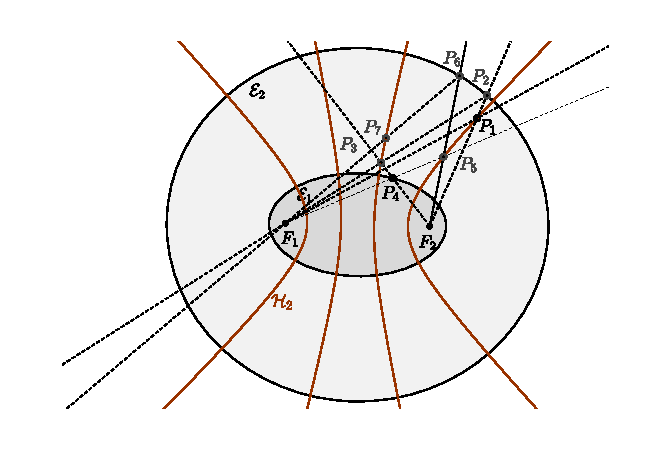
\includegraphics[scale=1]{ pics_08_910_dinamica_retangulos.pdf}
 		\caption {Sequence of points $P_1,  \,P_2, \ldots,  P_5 ,  \ldots$  
 		 \label{fig:retangulo_exerc82} }
 	\end{center}
 	\end{figure}
 	
 	\end{exercise}